\subsection{问题一}

\subsubsection{离散 Radon 变换模型}

CT(Computed Tomography)成像技术的核心数学基础是Radon变换。
Radon变换描述了如何将一个二维或三维对象的内部结构信息(如密度或吸收率分布)转换为其在各个方向上的投影数据。
它是一种将二维空间函数投影至其在线积分集合上的积分变换,
简单来说,就是一个物体映射在不同角度下的“投影”的集合。\par


Radon变换的基本物理定律是比尔-朗伯定律(Beer-Lambert Law),
该定律指出,当一束强度为 $I_0$ 的单色X射线穿过一个吸收介质后,
其出射强度 $I$ 会发生指数衰减。
衰减的程度取决于射线路径上各点吸收率 $f(x,y)$ 的线积分。其关系式为:

$$
I = I_0 \exp \left( - \int_L f(x,y) \, ds \right)
$$

对上式进行对数化,整理后可得投影数据 $p$ 与吸收率的线积分间存在直接关系:

$$
p = -\ln\left(\frac{I}{I_0}\right) = \int_L f(x,y) \, ds
$$

其中$L$ 代表单条X射线的路径,$ds$ 是路径上的线元。
题目附件二中提供的接收信息,正是经过处理后得到的投影数据 $p$ 的离散集合。

本文将此物理过程抽象为数学模型,已知二维断层切片的吸收率分布是一个二维函数 $f(x,y)$ ,
当一束平行的X射线以角度 $\theta$ 穿过,位于探测器坐标系中 $\rho$ 位置的探测单元所接收到的信号强度$p(\rho,\theta)$,
可通过Radon变换转化为函数 $f(x,y)$ 沿着直线 $x\cos\theta+y\sin\theta=\rho$ 的线积分,即:
$$p(\rho,\theta)=\int_{-\infty}^{\infty}\int_{-\infty}^{\infty}f(x,y)\delta(x\cos\theta+y\sin\theta-\rho)dxdy$$

其中 $\delta(\cdot)$ 是狄拉克函数,其性质确保了积分仅在指定的射线上进行。
仅当 $x\cos\theta+y\sin\theta=\rho$ 时,$f(x,y)$ 才对积分有贡献。\par

附件2的数据矩阵,每行代表一个固定的投影角度 $\theta_j$ ($j=1, \dots, 180$),
而每列的512个值则代表了在该角度下,沿不同位置 $\rho_i$ ($i=1, \dots, 512$) 的射线积分值。
附件2,即这个由所有投影数据构成的二维图像 $p(\rho,\theta)$ 被称为正弦图。\par

在实际的数字成像系统中,探测器单元数量有限,且待重建的吸收率函数 $f(x,y)$ 在离散的像素网格上表示。
因此,必须对连续的Radon变换模型进行离散化。

本文将积分运算近似为有限求和,并将狄拉克函数替换为其离散形式——单位脉冲序列$\delta[\cdot]$。
假设图像空间被离散为 $N \times M$ 的像素网格,则在第 $j$ 个角度 $\theta_j$ 下,第 $i$ 个探测器单元 $\rho_i$ 的投影值可以表示为:
$$p(\rho_i,\theta_j)=\sum_{k=1}^{N}\sum_{l=1}^{M}f(x_k,y_l)\delta[x_k\cos\theta_j+y_l\sin\theta_j-\rho_i]$$

在本问题中,图像网格大小为 $M=N=256$,探测器单元序号$i \in [1,512]$,扫描角度序号$j \in [1,180]$。

探测器单元的物理位置 $\rho_i$ 可定义为:

\begin{equation*}
\rho_i = i\Delta\rho, \quad i=1,2,\cdots,512 \\
\end{equation*}

取$\theta_0$ 为旋转前的初始角度,系统参数的离散化关系为:

\begin{equation*}
\theta_j = \Delta\theta_j + \theta_{j-1}, \quad j=1,2,\cdots,180
\end{equation*}



\subsubsection{探测单元间距的标定模型}

探测器单元间距 $\Delta\rho$ 的精确标定是后续图像重建的基础。
若物体在某一方向上的投影物理宽度为 $L$,该投影覆盖了 $N$ 个探测器单元,
则探测器单元之间的等效物理距离(即探测单元间距)$\Delta\rho$可表示为:

$$L = N \cdot \Delta\rho$$

为精确标定 $\Delta\rho$,我们分析了附件2中给出的模板投影数据(共180个角度)。
观察发现,这些数据呈现出两种显著的分布模式:单峰分布与双峰分布。

\begin{figure}[h] 
    \centering 
    
\includegraphics[width=0.8\textwidth]{圆形投影分离.png} 
    \caption{附件2数据分布标识图} 
    \label{fig:category}
\end{figure}

探测器单元接收值的可视化如图\ref{fig:category}所示:其中,黄色区域对应信号为零的探测器单元,
表明其接收路径上的X射线未穿过模板介质。
相对地,红色与蓝色区域标记了信号为非零的单元,说明X射线穿过模板(椭圆或圆或重叠部分)后被吸收而发生了衰减。

具体而言,单峰分布对应于X射线束在某些角度下同时穿过椭圆与圆形两个介质,导致它们的投影发生重叠;
而双峰分布则对应于射线束在另一些角度下分别穿过两个独立的介质,其投影在探测器上形成两个由零值区域隔开的非零信号区域。

为实现精确标定,必须利用一个尺寸已知的、在投影中易于识别的几何特征。
由椭圆的几何特性和圆的对称性可知,椭圆的投影宽度随扫描角度变化,而圆的投影宽度恒定。
因此,我们可以利用圆的投影宽度恒定这一特性来求解探测器间距。
因此模板中的圆形介质是一个理想的标定参照物,其在在任意角度下的投影宽度恒为其直径,
即 $L_c = d_c = 4 mm$。

由于圆形的尺寸远小于椭圆,因此其投影宽度也相应较窄。
很容易可以从双峰分布的投影数据中,精确分离出仅由圆形介质产生的投影信号段
(即图\ref{fig:category}中的红色部分),
然后利用其投影宽度与对应的探测器单元数来求解 $\Delta\rho$。

对于每一个被识别出的圆形有效投影,统计其覆盖的探测器单元数量,记为 $N_i$,其中 $i$ 是有效投影的索引。
由于实际数据中可能存在噪声和离散化误差,直接使用单次测量值不够稳健,
为提高标定结果的精度和鲁棒性,对所有筛选出的 $k$ 个有效投影宽度 $N_1, N_2, ..., N_k$ 求取算术平均值,:
\begin{equation}
    \bar{N} = \frac{1}{k} \sum_{i=1}^{k} N_i
    \label{eq:average_N}
\end{equation}



\subsubsection{投影宽度的解析模型}
将模板整体模拟成一个二维平面内的系统,
由一个中心位于原点、长轴为 $a$、短轴为 $b$ 的椭圆和一个半径为 $r$、圆心位于 $(m, 0)$ 的圆构成。
\begin{figure}[h] 
    \centering 
    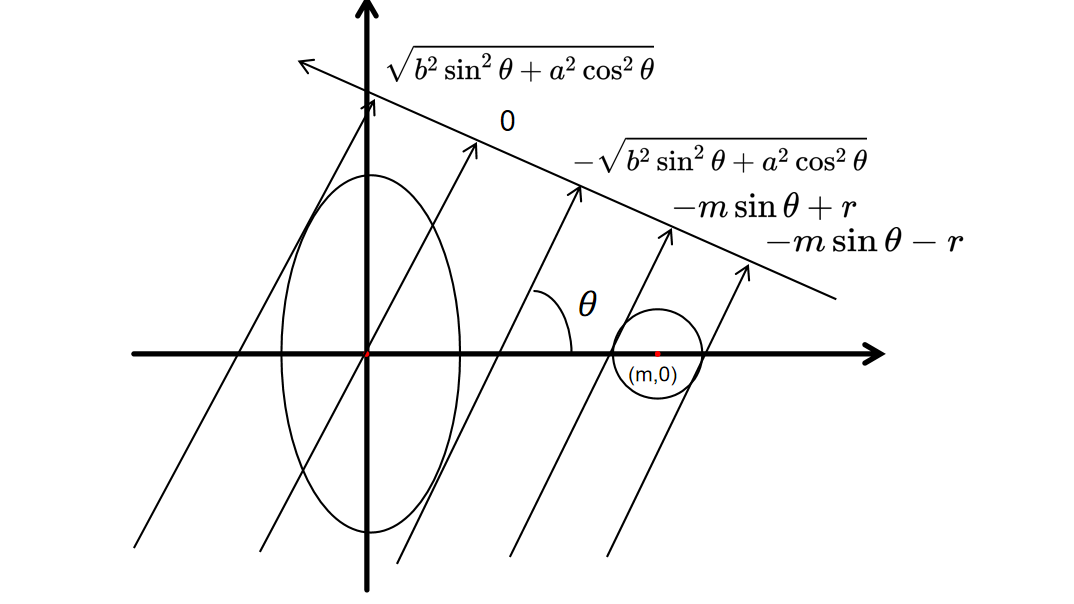
\includegraphics[width=0.8\textwidth]{几何图.png} 
    \caption{投影几何示意图图} 
    \label{fig:category}
\end{figure}

如上图所示,当一束与水平方向成夹角 $\theta$ 的平行光照射该模板时,两个图形将在垂直于光线方向的探测器平面上形成阴影。
设光线方向的单位向量为 $\mathbf{d} = (\cos\theta, \sin\theta)$,
则垂直于光线的探测器方向为单位向量 $\mathbf{n} = (-\sin\theta, \cos\theta)$。

椭圆在探测器方向上的投影为对称区间,其半宽度为:
\[
w_e(\theta) = \sqrt{b^2 \sin^2\theta + a^2 \cos^2\theta}
\]

圆心在投影方向上的坐标为:
\[
p_c = -m \sin\theta
\]

其对应的投影区间为 $[p_c - r,\ p_c + r] = [-m \sin\theta - r,\ -m \sin\theta + r]$。将椭圆和圆在探测器方向上的投影视为两个区间,则它们的总阴影长度为这两个区间的并集长度。可以统一表示为如下解析表达式:
\begin{equation}
\begin{split}
L_{\text{total}}(\theta) =\ & \max\left( \sqrt{b^2 \sin^2\theta + a^2 \cos^2\theta},\ -m \sin\theta + r \right) \\
& - \min\left( -\sqrt{b^2 \sin^2\theta + a^2 \cos^2\theta},\ -m \sin\theta - r \right)
\end{split}
\end{equation}



